%!TEX root = main_ISMB.tex
\section{Results}
\label{sec:results}

\subsection{Implementation}
\label{sec:implementation}
Our software, \ourprog, was implemented in {\tt Python~2.7}. We used
\RNAinverse from the \textit{Vienna Package 2.0}~\citep{Hofacker:1994}.
All time benchmarks were run on a single AMD Opteron(tm) 6278 Processor  at 2.4 GHz with cache of 512 KB.
The penalty $\beta$, associated with invalid base-pairs, was set to $15$.

\begin{figure}[ht!]
	\centering
 	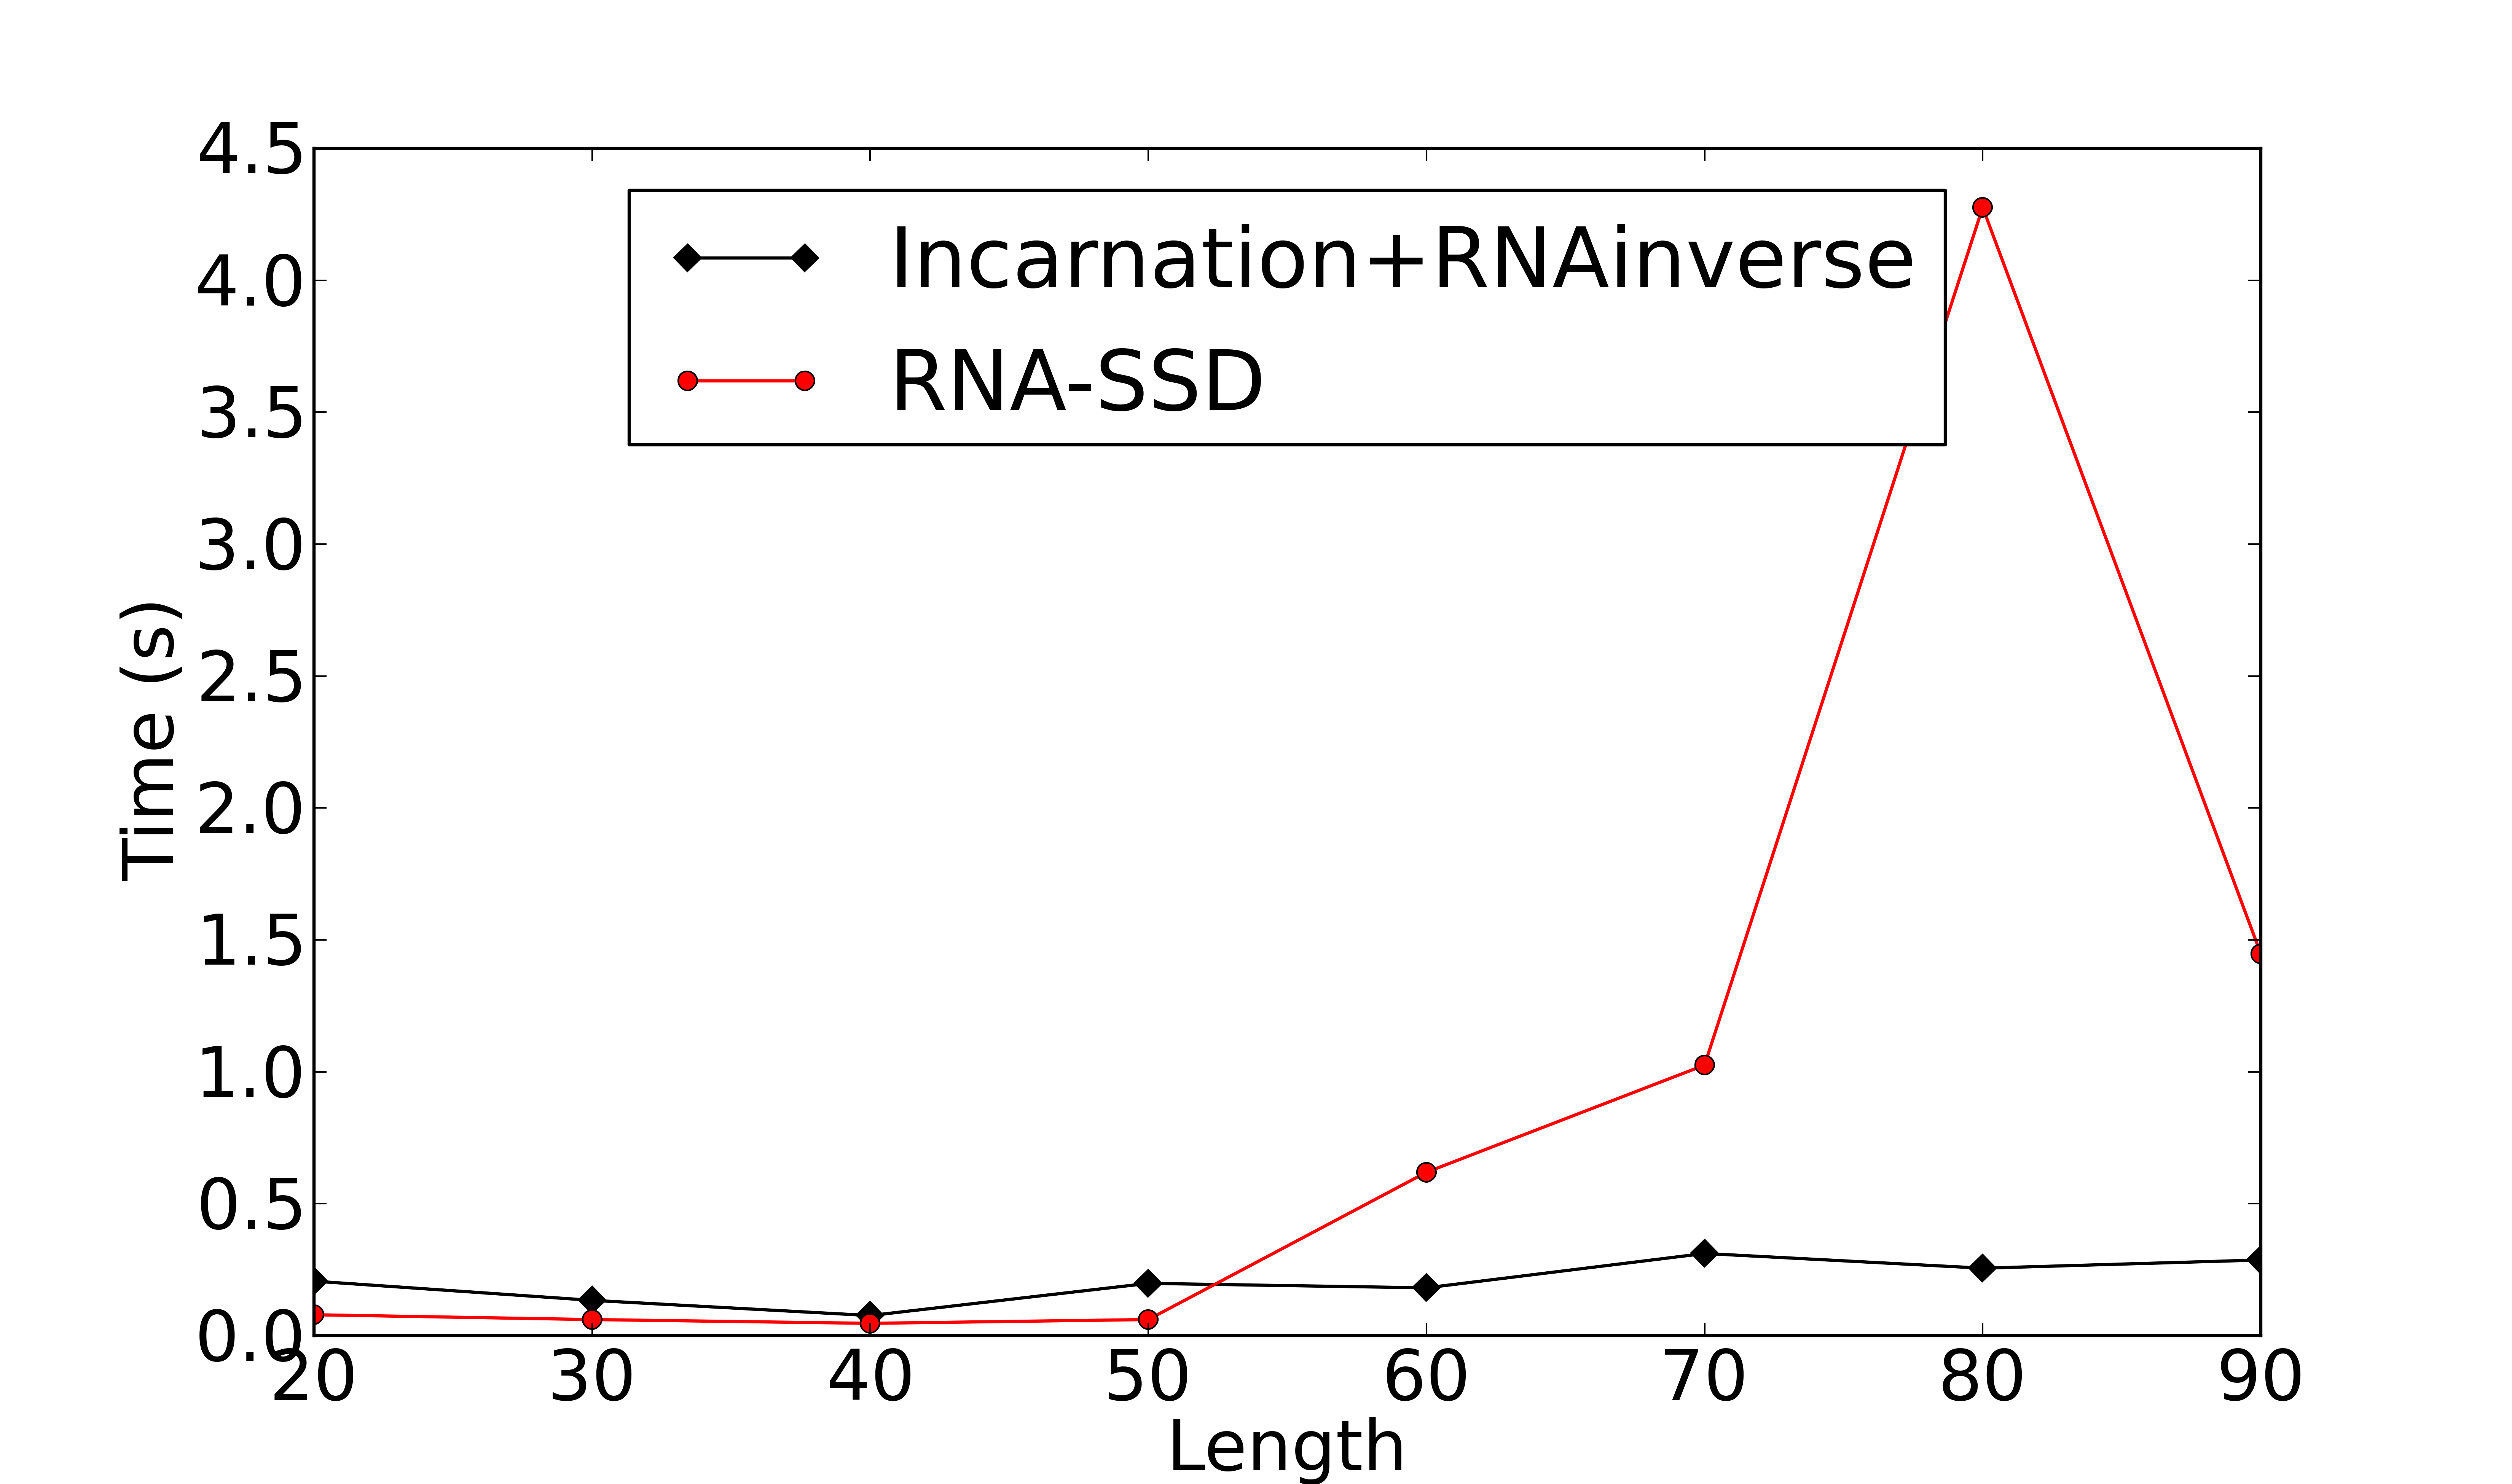
\includegraphics[width=0.5\textwidth]{Figures/time_incar_rnassd}
	\caption{
  Average time in seconds to generate one sequence for \ourprog and \RNAinverse.}
	%the time spent by \ourprog (full line) and \texttt{RNAinverse} (dashed) for various \GCContent. The first plot is in function
	%of the length of the structures. The second is in function of the stack
	%density (i.e. $2\cdot\#stacks/length$) and the latter in function of 
	%the proportion of free nucleotides (i.e. unpaired bases) within loops.}
	\label{fig:time}	
\end{figure}

Figure~\ref{fig:time} presents the average times spent running \ourprog and \RNAinverse to generate one sequence
with the required \GCContent. As expected, the time grows linearly
in function of the length of the structures for \ourprog.  A highly intriguing feature is the substantial decrease of the time 
required for running \RNAinverse when $15\%$ of nucleotides are unpaired in the target structure.
However, one must remain careful interpreting this observation, as the structures within this class all originate from the PDB, and are relatively small (for the complete STRAND DB, the average length is $\sim526$nts, compared to $\sim38$nts around 15\% unpaired bases).



\subsection{Dataset}
To evaluate the quality of our method, we used secondary
structures from the \RNASTRAND database~\citep{andronescu2008rna}.
Those are known secondary structure from a variety of organisms.
We considered a subset of $50$ structures selected by~\cite{Levin:2012kx}, 
whose length ranges between $20$ and $100$ nucleotides. 
To ease the visualization of results, we clustered together structures
having similar length, stacks density and proportion of free nucleotides in loops,
leading to distributions of structures shown in Figure~\ref{fig:bins}.

 \begin{figure*}[ht!]
 	\centering
	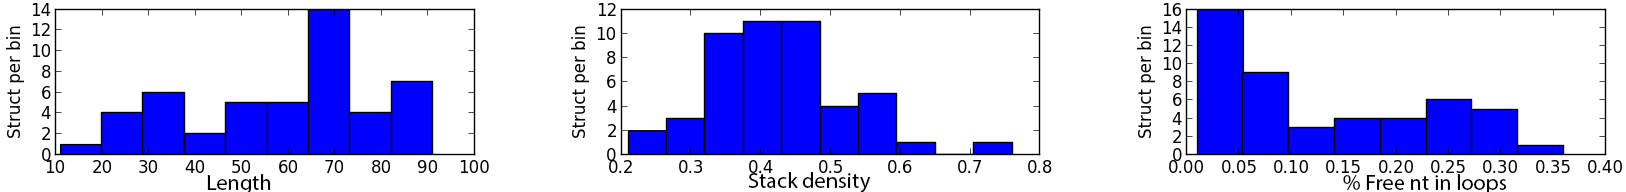
\includegraphics[width=\textwidth]{Figures/bins_distribution.png}
	\caption{Number of secondary structures per bin, according to our three clustering criteria.}
	\label{fig:bins}
 \end{figure*}
 
 \highlight{
\subsection{Design}
We ran our method as follows. First, we sampled approximately $100$ sequences per structure. Then, we use these sequences 
as seed in \RNAinverse. Finally, we computed the MFE with the \rnafold program from the \textit{Vienna Package 2.0} \citep{Hofacker:1994}.

Before starting our benchmark, we asses the need for our methods and performed an analysis of the \GCContent drift achieved with state-of-the-art software. Using our dataset of $50$ structures, we generated $100$ samples per structure with classical softwares who do not control the \GCContent. Namely,  \RNAinverse, \INFORNA, \NUPACK and \frankenstein.  We show the distribution of the \GCContent of the sequences produced with these softwares in Fig.~\ref{fig:gcdist} those distributions.

As anticipated, we observe a clear bias toward high {\GCContent}s and a complete absence of sequence with less than $30\%$ of \GC. This striking results motivates a need for methods that enable to explicitly control the \GCContent and more precisely that enable to design sequences with low \GCContent (i.e. 30\% or less). In order to provide a complete overview of the performance of \ourprog, we provide additional statistics for these software in the supplementary material.
}

\begin{figure}[ht!]
  \begin{center}
    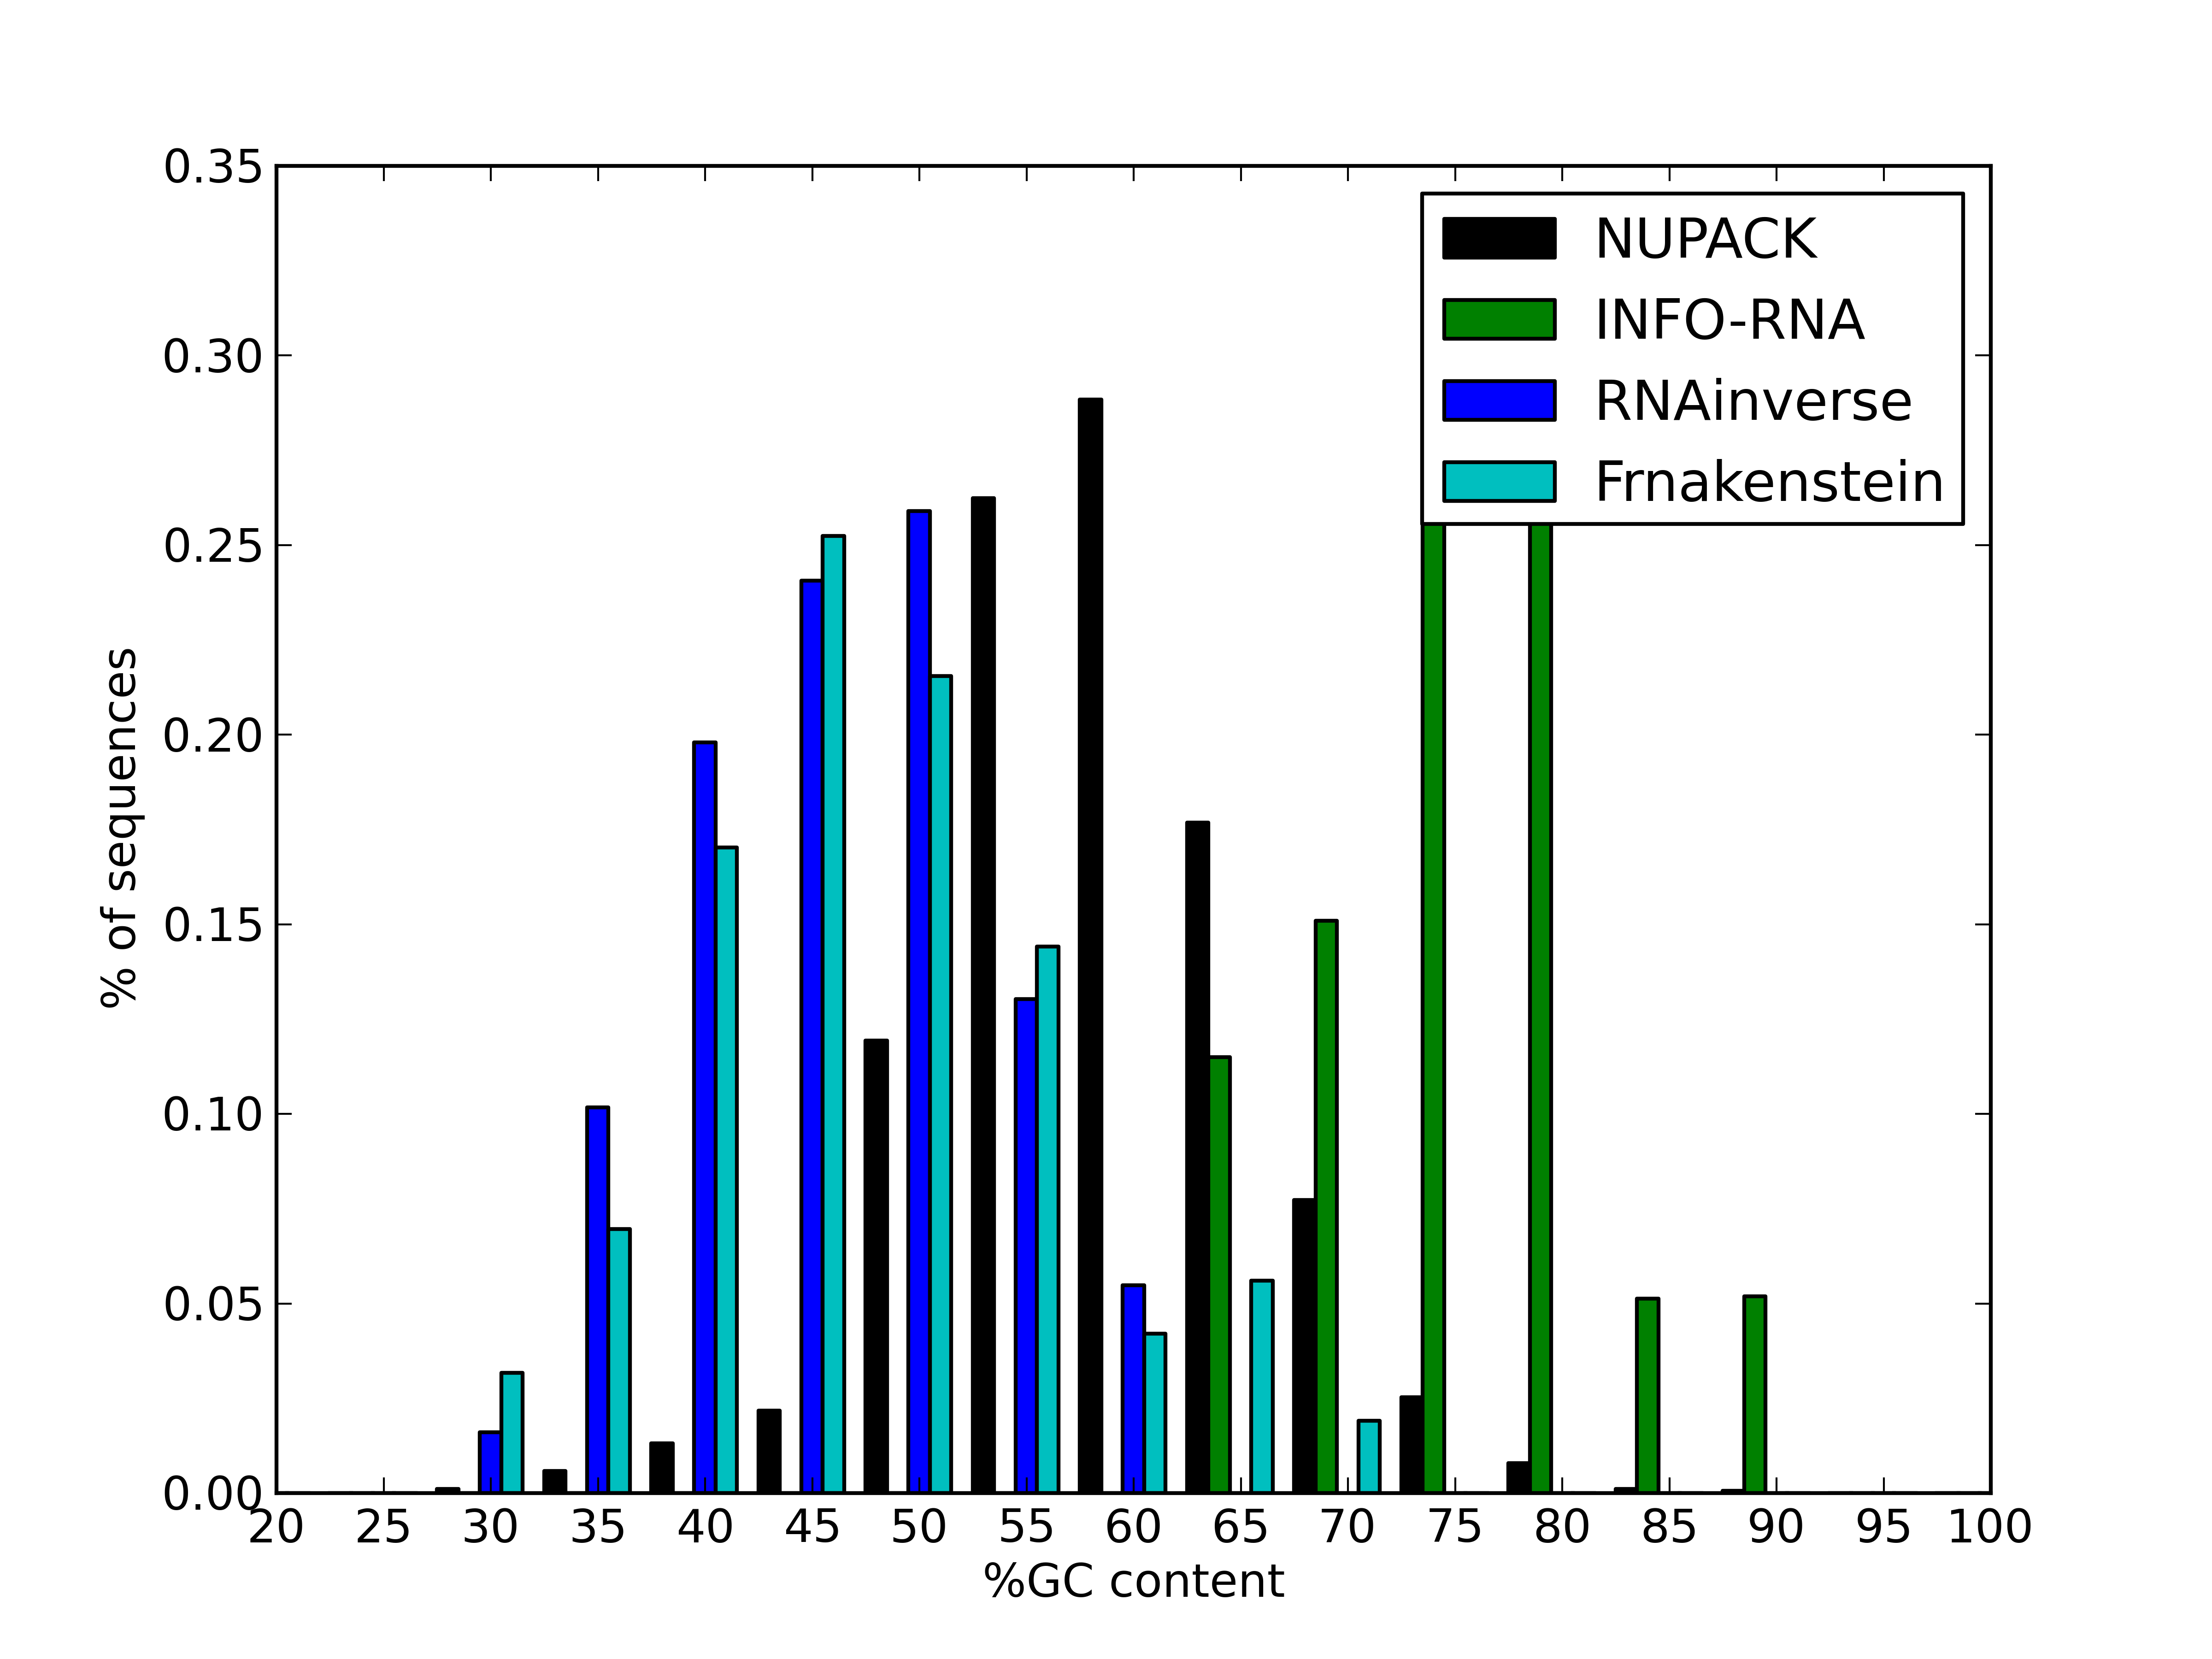
\includegraphics[width=0.5\textwidth]{Figures/histograme_5_gc_distribution_nornaexinv.png}
  \end{center}
  \caption{Overall \GCContent distribution for sequences designed using \RNAinverse, \INFORNA, \NUPACK and \frankenstein folding in the desired structure.}
  \label{fig:gcdist}
\end{figure}

\highlight{
\subsection{Success rate}
We started by estimating the success rate of our methodology and computed the percentage of sequences with a MFE structure identical to the target secondary structure. Figure~\ref{fig:mfe_struct_solved_noinverse} shows our results. We clearly see that before the post-processing step (i.e. \RNAinverse) the sequences sampled by \ourprog have a low success rate (first row). As mentioned earlier, this could be explained by the fact that no selection criterion has been at this stage applied to unpaired nucleotides. Remarkably, after the local search optimization (with \RNAinverse) of nucleotides in unpaired regions (second row), we observe a dramatic improvement of our success rate. As expected, we observed that length is, in general, not a good predictor for the hardness of designing a structure. Instead, a high number of free nucleotides in the structure seems to be a  good measure of the hardness of its design. Similarly, these data also show that designing sequences with low \GCContent is challenging for all types of targets.
}

\begin{figure*}[ht!]	
	\centering
	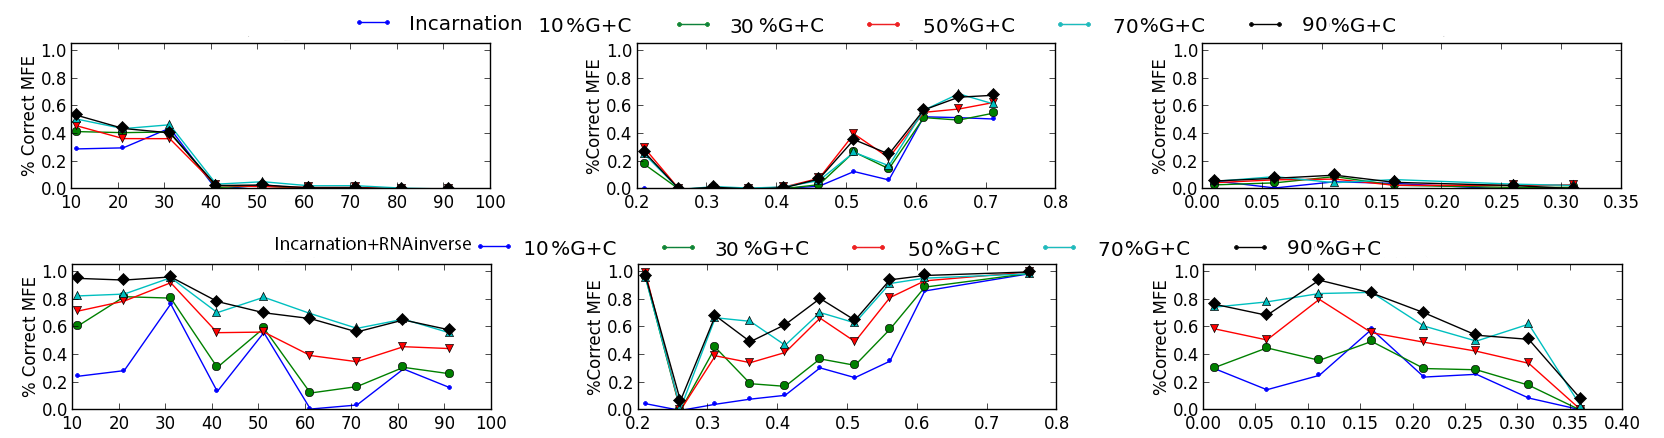
\includegraphics[width=\textwidth]{Figures/mfe_struct_solved_vsrnainverse}
	\caption{Success rate \ourprog before after after \RNAinverse post-processing. The first row shows the percentage of sampled sequences folding into the target when using only \ourprog. The second shows after processing previous results with \RNAinverse.}
	\label{fig:mfe_struct_solved_noinverse}	
\end{figure*}



%\begin{figure*}[ht!]	
%	\centering
%	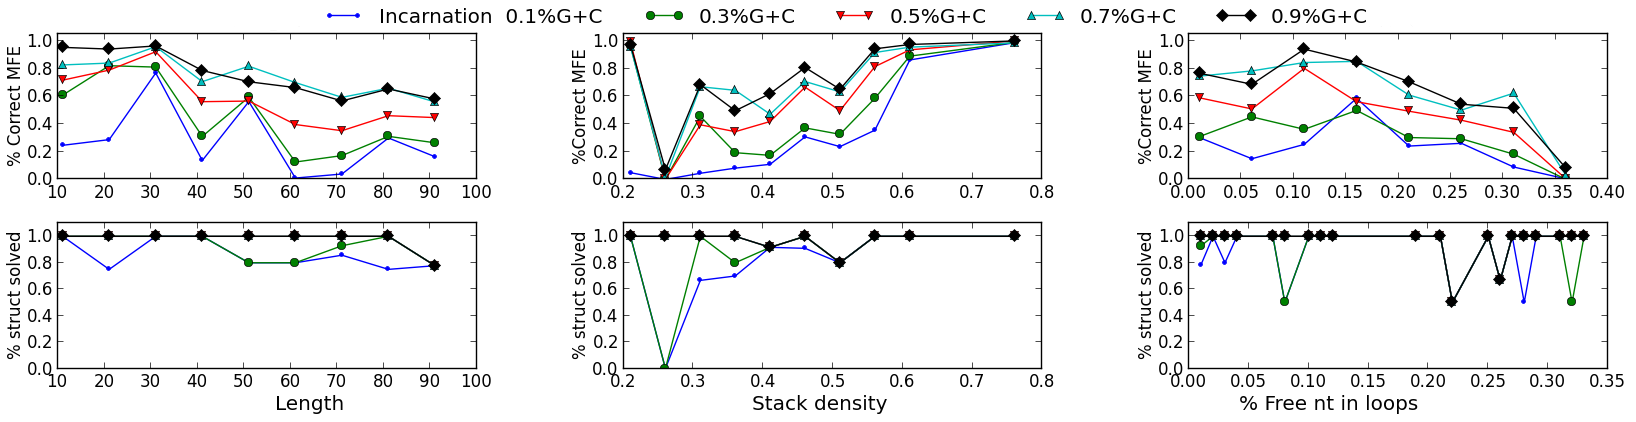
\includegraphics[width=\textwidth]{Figures/mfe_struct_solved}
%	\caption{Quality of \texttt{Incarnation+RNAinverse} results. The first row shows the percentage
%	of sampled sequences folding into the target. The second shows the 	
%	proportion	of structures for which at least one correct sequence was 
%	sampled.}
%	\label{fig:mfe_struct_solved}	
%\end{figure*}

\highlight{ 
We investigated further the quality of the sequences generated by \ourprog. In particular, we estimated the capacity of our methods to generate ``good'' sequences with desired folding capabilities regardless of the property  to fold exactly into the target structure. In Figure~\ref{fig:ss_sens}, we show the ratio of well predicted base pairs in the MFE structure of our sampled sequences. As above, we can observe that, in all cases, the sequences that are the hardest to design are those with an extremely low \GCContent. Indeed, the energetic contribution of the base pairs to the stability of the structure is weaker. Interestingly, we also notice that the most accurate sequences yield a \GCContent of $70\pm 10\%$. Overall, we observe that all our samples have good folding properties, and that there is a correlation between the ``precision'' of the samples and the hardness of the design.
}

As discussed in Sec.~\ref{sec:implementation}, we noticed a highly decreased computational time needed to generate the sequences with $15\%$ free 
nucleotides in the loops. We remark that those structures also yield a much lower structural sensitivity.

\begin{figure*}[ht!]
 	\centering
	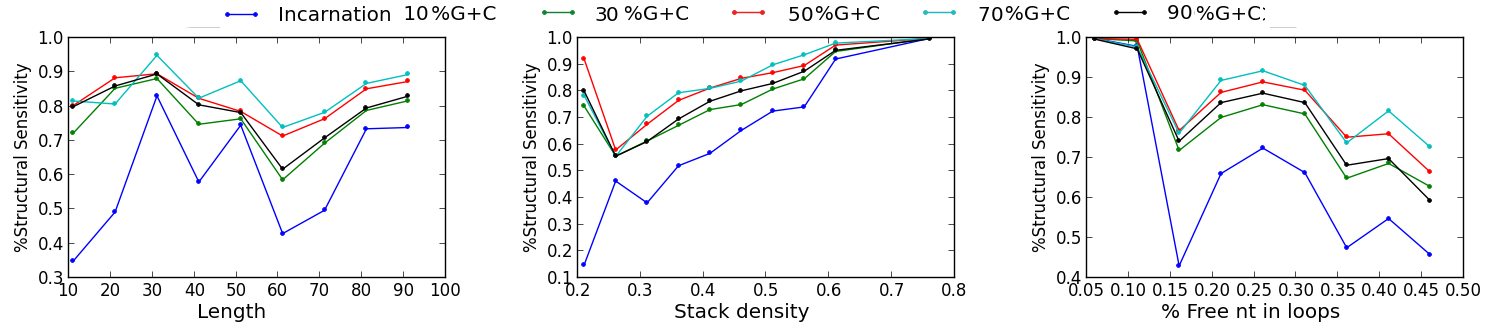
\includegraphics[width=\textwidth]{Figures/rnastrand_clustered_rnainverse_100samples_struct_sens.png}
	\caption{Structural sensitivity (i.e. $\#$ well predicted base pairs / $\#$ base pairs in target) of the sampled sequences MFE. }
	\label{fig:ss_sens}	
\end{figure*}

\subsection{Properties of designed sequences}

In this section, we further analyze the generated sequences with a MFE structure that folds into the target structure. 

%The positional entropy is defined as:
%\begin{align}
%  \sum_{\substack{i\\b \in (\Ab,\Cb,\Gb,\Ub)}} -p_{i\to b}\cdot \log_4(p_{i\to b}) &&& \text{(Positional entropy)}
%  \label{eq:entropy}
%\end{align}
%where $p_{i\to b}$ is the proportion of nucleotides $b$ at position $i$.
%Intuitively, this measure captures the variability of sequences generated by a given method.

\highlight{
A desirable feature in sequence design, is to produce samples with a high sequence diversity and stable secondary structure. 
Therefore, in the following we will use two useful measures which are the sequence identity of the samples, and the Boltzmann probability
of the target structure in the low energy ensemble.

The sequence identity is defined over a set $\mathcal{S}$ of aligned sequences (in our case, all sequences have the same length and can be trivially aligned) as :
\begin{align}
  \sum_{s^1,s^2 \in\mathcal{S}\times\mathcal{S}}\left(\frac{1}{|s^1|}{\sum_{\substack{i\\s^1_i\equiv s^2_i}}1}\right) &&& \text{Seq. identity}
\end{align}
where $s_i$ is the nucleotide at position $i$ in sequence $s$. Intuitively, this measure captures the diversity of sequences generated by a given method. Next, the Boltzmann frequency is defined, for a structure $\Struct$ and a sequence $s$ as:
\begin{align}
  e^{\frac{-\ES(s,\Struct)}{RT}}/\mathcal{Z}^s  &&&\text{Frequency}
\end{align}
where $\mathcal{Z}^s$ is the partition function of sequence $s$. This measure tells us how dominant is a structure $\Struct$ in the Boltzmann ensemble of structure over a sequence $s$. A high value implies a stable structure. We compute this frequency with \rnafold from the \texttt{Vienna Package 2.0} \citep{Hofacker:1994}.
}

%The base pair entropy is defined as:
%\begin{align}
%  \sum_{i<j}-p_{i,j}\cdot \log_2(p_{i,j})&&& \text{(Base-Pair entropy)}
%  \label{eq:bpentropy}
%\end{align}
%where $p_{i,j}$ is the Boltzman probability, i.e. probability that a random structure drawn with respect to 
%the Boltzmann distribution forms a base-pair between positions $i$ and $j$. The base pair entropy reflects
%the distribution of structures weights in the Boltzmann ensemble. Thus, a low base pair entropy implies a highly conserved structure.
%To compute the base pairs probabilities, we used \rnafold from the \texttt{Vienna Package 2.0} developed by~\cite{Hofacker:1994}.

%Figure~\ref{fig:nb_sols_entropy} shows the number of correct solutions as their average entropy and positions inside base pairs entropy, since \ourprog  only influences the distribution of nucleotides inside stacked base pairs. The most constraining factor for generating valid solutions seems to be  low \GCContent and the percentage of free nucleotides. 

\highlight{
Figure~\ref{fig:nb_sols_entropy} shows the number of solutions generated (i.e. sequences with a MFE structure identical to the target structure) and the average sequence identity of the sequences. Here, we note that low {\GCContent}s have a strong (negative) influence on the number of sequences generated, and in parallel also affect negatively the sequence diversity. This observation emphasizes the difficulty to  design sequences with low \GCContent. Once again, large percentages of free nucleotides increase the difficulty of the task. 

The thermodynamical stability of the target structure on the designed sequence is another important property when estimating the performance of RNA design algorithms. We estimate the quality of our solutions in Figure~\ref{fig:freq}. First, we observe a slow decline of the structure stability (i.e. the frequency) when the target structure increases in size. Yet, for an average \GCContent, the frequency stays over $10\%$ even at size of $100$ nucleotides. Next, we note that for the most difficult target structures (i.e. the longer ones or those with high percentages of unpaired nucleotides in loops) the \GCContent have a limited (almost null) influence on the stability of the target structure on the designed sequence. By contrast, this less true for easiest and small structures with only few free nucleotides in internal loops.
}

\begin{figure*}[ht!]
	\centering
	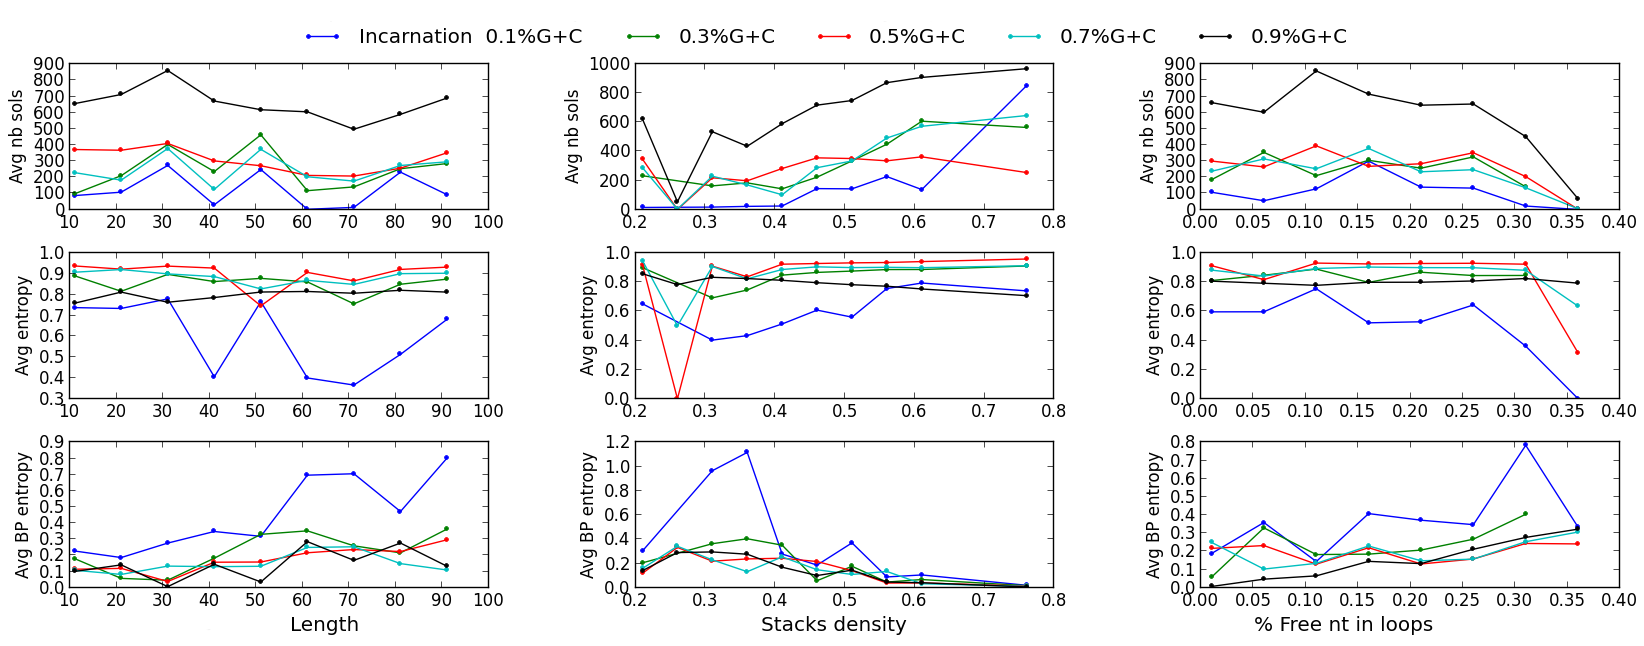
\includegraphics[width=\textwidth]{Figures/nb_sols_entropy}
	\caption{Number of solutions generated by \ourprog and their average sequence identity. The curves are parameterized by the {\GCContent} of the sequences. The data are plotted vs. the length of the target (left), density of stacked base pairs (centre) and number of unpaired nucleotides  in loops (right).}
	\label{fig:nb_sols_entropy}
\end{figure*}


\begin{figure*}[ht!]
	\centering
	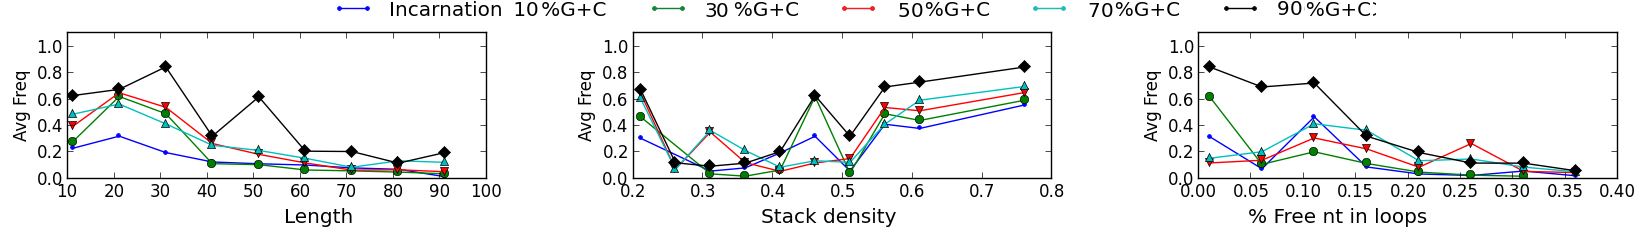
\includegraphics[width=\textwidth]{Figures/freq.png}
	\caption{Thermodynamical stability of the target structure. The curves report the average Boltzmann probability of the target structure (which is also the MFE structure) at various {\GCContent}s w.r.t. the length of the target (left), density of stacked base pairs (centre) and number of unpaired nucleotides  in loops (right).}
	\label{fig:freq}
\end{figure*}

\highlight{
\subsection{Global sampling vs Local search vs Glocal approach}
To conclude this study, we estimate the impact of the design methodology on the performances. More precisely, we aim to determine the merits of a global sampling approach (\ourprog), compared to a glocal procedure (\ourprog + \RNAinverse) and a local search methodology (\RNASSD). To our knowledge, \RNASSD, beside \ourprog, is the only software that implements an explicit control of the \GCContent.

Here, we compare the running time and the sequence diversity of the solutions produced by each software. In addition, we focus on the design of sequences with low {\GCContent}s (30\% and less) as they are almost impossible to design with classical software (See Figure~\ref{fig:gcdist}).

Figure~\ref{fig:time} shows the running time of each software. These data demonstrate the efficiency and scalability of our techniques. In particular, this figure suggests that our strategy has the potential to be applied efficiently for designing sequences on long (and difficult) target secondary structures at low \GCContent -- A task that could have not been achieved before due time requirements.

Next, we show in Figure~\ref{fig:benchmark_RNASSD} the average sequence identity achieved by the various methods. Our results show that at extremely low {\GCContent}s (i.e. 10\%), \ourprog slightly outperforms \RNASSD while this advantage becomes less evident when the \GCContent increases. Our experiments on higher {\GCContent}s (i.e. 50\% and above) showed that our glocal strategy and the local search approach perform similarly. Similarly, we did not find any clear evidence that a global, local or glocal approach outperforms others when we compare at the thermodynamical stability of the target structure (data not shown).
}

\begin{figure*}[ht!]
  \centering
  \includegraphics[width=\textwidth]{Figures/seq_identity_10_30}
  \caption{Sequence identity of \ourprog and \RNAinverse for $10$ and $30\%$ of \GC.}
  \label{fig:benchmark_RNASSD}
\end{figure*}



% \ourprog outperforms other strategies for non-centered . In particular, the base pair entropy as well as diversity of sequences are favorable to \ourprog. This advantage is even more striking for low targeted \GCContent{}s regimes.
%To complete this benchmark, we added the results obtained with the glocal procedure (\ourprog + \RNAinverse). We note that the results are slightly lower than those of \ourprog alone. However, we must stress that the \ourprog data consider only the sample of \ourprog already satisfying the MFE criterion. In fact \RNAinverse enable to ``correct'' a lot of sample sampled by \ourprog but without the good folding properties. Hence, our conclusion here is that the glocal approach enable us to conserve the same level of performance but to drastically improve the success rate of our methodology. 






%\label{fig:rnainverse}

